This section covers a variety of experiments and situations to test the applicability of the planners on each of the problem generated by the problem generators looked at within this report. The notation $PL$ is used when referring to the number of program lines used to represent a generalised plan.

\section{Effect of Varying Tile Sizes}
As mentioned throughout this report, the variable $T$ is used to denote the tile size, which is the number of tiles that can fit on a row on the display. In this report, the maximum size of any board is given by $T^2$. As $T$ increases, there problems in all domains become more complex, involving the agent having to locate larger paths. These experiments will observe the effects of varying $T$ to demonstrate the impact larger boards have on the runtime of the generators and the planners. These tests will look into the runtime of generators when tasked with compiling 5 problems for each value of $T$ where the $T$ ranges from 2 to 30.

\subsection{Classical Planning}
The average trend seen in generators, where one object directly correlates to a single object, was exponential, which is shown in Figure 4.1. For the Directional problem generator, on small problems, the plans were generated on quickly. As the complexity increases rapidly due to the number of objects imposed on large environments, the planner would fail to solve plans in a reasonable time frame (60 seconds), hence it is not included in the results. The time it takes to generate the problems is usually negligible ($\leq 1s$) and is the same for all generators, even the Directional problem generator. Overall, using classical planning on a problem set of reasonable scale ($T \leq 30, |\mathcal{P}| \leq 5$), solutions under 60s can be expected. The dips seen in Figure 4.1 are due to the generator creating simpler problems on average, over the 5 problems at that setting of $T$, over each of the generators.

\subsection{Generalised Planning}
However, when attempting to find general solutions, $|P|$ was only solvable for smaller values of $T$ in the generators where the problem had been reduced. For the initial Maze and the Snake problems, the planner could not find a solution in any number of program lines $\leq 100$ in a reasonable time frame. In an experiment containing 3 problems where $T = 5$, using the Directional problem generator, a generalised solution was created in 9,780 seconds (2 hours, 43 minutes). This is almost 3000 times the time it took for the classical planner to solve 5 problems of that scale. For smaller problems however $T = 2, 3$, the generalised planner found solutions to most problems in all the domains in under a 1 second. This is most likely due to the fact that generated problems of this size shared many common features, so the BFGP was able to exploit this to generate a solution rapidly.

\subsection{Mean Runtime Trend}
\begin{figure}[h!]
    \centering
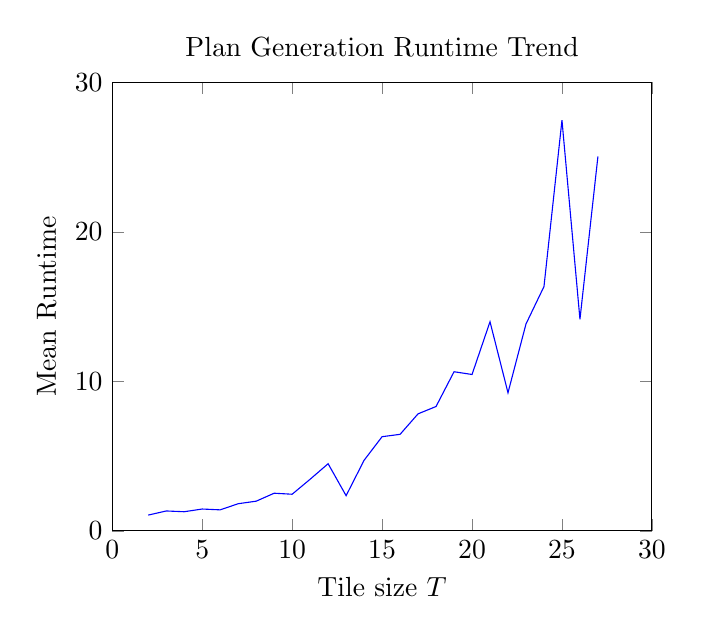
\begin{tikzpicture}
\begin{axis}[
    title={Plan Generation Runtime Trend},
    xlabel={Tile size $T$},
    ylabel={Mean Runtime},
    xmin=0, xmax=30,
    ymin=0, ymax=30,
]

\addplot[
    color=blue,
    ]
    coordinates {(2, 1.0514459609985352)
(3, 1.327857494354248)
(4, 1.2770888805389404)
(5, 1.4581902027130127)
(6, 1.402270793914795)
(7, 1.8123571872711182)
(8, 1.9829325675964355)
(9, 2.51538348197937)
(10, 2.4477152824401855)
(11, 3.4509198665618896)
(12, 4.489059686660767)
(13, 2.3502399921417236)
(14, 4.71928334236145)
(15, 6.297330141067505)
(16, 6.456403493881226)
(17, 7.827086925506592)
(18, 8.318503856658936)
(19, 10.644485712051392)
(20, 10.46013331413269)
(21, 13.989691734313965)
(22, 9.238670349121094)
(23, 13.84094762802124)
(24, 16.344945669174194)
(25, 27.47840189933777)
(26, 14.154968738555908)
(27, 25.057862758636475)};
    
\end{axis}
\end{tikzpicture}
\caption{Runtime on the generation of plans with increasing $T$}
\end{figure}

\subsection{Evaluation}
Overall, the generalised planner took exponentially more time to arrive at a solution than the classical planner where $T \geq 3$, most likely due to the lack of similarities between problems within $\mathcal{P}$. This was the case for all problems generated by any problem generator, except the problems created from a problem reduction were solved significantly faster.

\section{Comparative Analysis of Maze Problems}
This experiment involves comparing the runtime of the BFGP++ generalised planner on a fixed set of problems generated by the various problem generators mentioned within this report. For this, the tile size will remain constant at $T=5$ and each problem set $\mathcal{P}$ will contain 3 problems. An mean runtime will be taken over a set of 5 problem sets, the images of these Maze problems will be given in the Appendix. 

\subsection{Problems with No Turns}
This first set of problem sets contains Maze problems that contain no turnings that the agent has to make. This experiment aims to determine whether the absence of actions that involve re-orientating the agent will have an effect on the performance of the planner. The results generated in this experiment is given below:

\begin{table}[ht]
\centering
\begin{tabular}{|p{0.25\linewidth}|p{0.09\linewidth}|p{0.09\linewidth}|p{0.09\linewidth}|p{0.09\linewidth}|p{0.09\linewidth}|p{0.12\linewidth}|}
\hline
Problem Generator & $\mathcal{P}_1$ & $\mathcal{P}_2$ & $\mathcal{P}_3$ & $\mathcal{P}_4$ & $\mathcal{P}_5$ & Mean \\\hline
Maze & DNF & DNF & DNF & DNF & DNF & DNF
\\\hline
Directional Maze & 0.1s & 0.1s & 0.3s & 0.3s & 0.3s & 0.22s
\\\hline
Non-Directional Maze & 2.6s & 0.02s & 0.7s & 0.4s & 0.03s & 0.75s
\\\hline
\end{tabular}
\caption{Results for the "Problems with No Turns" experiment}
\end{table}

\subsubsection{Evaluation}
Surprisingly, although there were no turning actions involved, the generalised planner could not find a solution in a reasonable time frame (60s) to solve a single problem. Even more surprisingly, is that on average the Non-Directional problem generator took more that double the amount of time for the same set of problems. Excluding the outlier of 2.6s, the average would be 0.23s which is still higher than the average taken in the Directional Maze problems. This could be the case as there are multiple solutions in each method used to solve the Directional problems, due to its structure. This could lead to the planner being able to observe a variety of states which correspond to the same real-world action, simplifying the number of states required to search for a solution. 

\subsection{Identical Problems}
This second set of problem sets contains Maze problems that are identical to each other within the set. These problems can contain turns. I hypothesise that the generalised planner will be able to compute a solution almost instantly in all problem generators as all the problems share similarities. Shown below is the results of this experiment:

\begin{table}[ht]
\centering
\begin{tabular}{|p{0.25\linewidth}|p{0.09\linewidth}|p{0.09\linewidth}|p{0.09\linewidth}|p{0.09\linewidth}|p{0.09\linewidth}|p{0.12\linewidth}|}
\hline
Problem Generator & $\mathcal{P}_1$ & $\mathcal{P}_2$ & $\mathcal{P}_3$ & $\mathcal{P}_4$ & $\mathcal{P}_5$ & Mean \\\hline
Maze & 0.1s & DNF & DNF & DNF & DNF & DNF
\\\hline
Directional Maze & 0.1s & 0.3s & 0.6s & 1.4s & 1.8s & 0.84s
\\\hline
Non-Directional Maze & 0.02s & 0.03s & DNF & DNF & DNF & DNF
\\\hline
\end{tabular}
\caption{Results for the "Identical Problems" experiment}
\end{table}

\subsubsection{Evaluation}
In all cases, the generators were able to solve the identical problems containing a straight line, almost instantly. However, in cases where there was a turn the Maze generator started falling off, failing to produce a solution in a reasonable time frame. Oddly, for problem sets containing two or more turns, the planner started to fail on the Non-Directional Maze problems. Overall, the only generator that passed every test was the Directional Maze generator, which was able to handle all the problem sets.

\subsection{Analysis on the Effect of the Maze Problem Reduction}
For a set of problems that share no similarities between them, problems with the initial Maze domain were too complex for the generalised planner to solve them. As the domain only contains a single action after the reduction, the generalised planner only focuses on where to put a move action rather than having to orientate the agent. This takes up significantly less program lines in the resultant generalised solution as well. Furthermore, the generalised planner can generate plans at a similar rate regardless if there is a turning in the Maze. To put it into perspective, the problems in set in Figure 3.15 would take roughly the same amount of time if they are generated by either generator. If any problem in that set contained a turning, it would take exponentially more time for the planner to solve it, if that problem was generated on the initial Maze domain. In either the Directional or Non-Directional problems, there would be almost no change.\\\\
Overall, in all experiments, plans generated on problems created in the Directional Maze problems, yield the best results. It was able to handle instances where there were little similarities, as well as being able to handle the orientation of the agent in problems that involved turns.

\section{Aside: Efficiency of Generalised Solutions}
This aside experiment will explore a point of interest that came up during the development of this project. Although this is proven incorrect later, it still provides some insight to those interested in the field. This experiment involves measuring the efficiency of solutions generated by a generalised plan $\Pi$. The measure of \textit{inefficiency} $\overline{E}$ of a generalised solution is given by the cost of the classical plan generated through classical planning divided by the cost of the classical plan generated through generalised planning.

\subsection{Hypothesis}
\textit{There is a relationship between the efficiency of a solution and the number of program lines available to the generalised planner.} When the planner is limited to small number of program lines $PL \leq 15$, the solutions tend to be more inefficient as seen in Figure 3.16. If a classical planner can solve the same problem in 3 lines, the inefficiency score of generalised solution given in Figure 3.16 is $\frac{8}{3} = 2.\dot{6}$. In this report, a plan is \textit{efficient enough} if $\overline{E} \leq 1.5$. Figure 4.3 shows the relationship between the mean inefficiency score $\frac{\Sigma\overline{E}}{|\mathcal{P}|}$, over the set of problems $\mathcal{P}$, and the number of program lines $10 \leq PL \leq 50$ in the synthesis of generalised plans for the following set of problems shown in Figure 4.2. This experiment uses the Directional problem generator to generate the three problems.

\begin{figure}[h!]
    \centering
    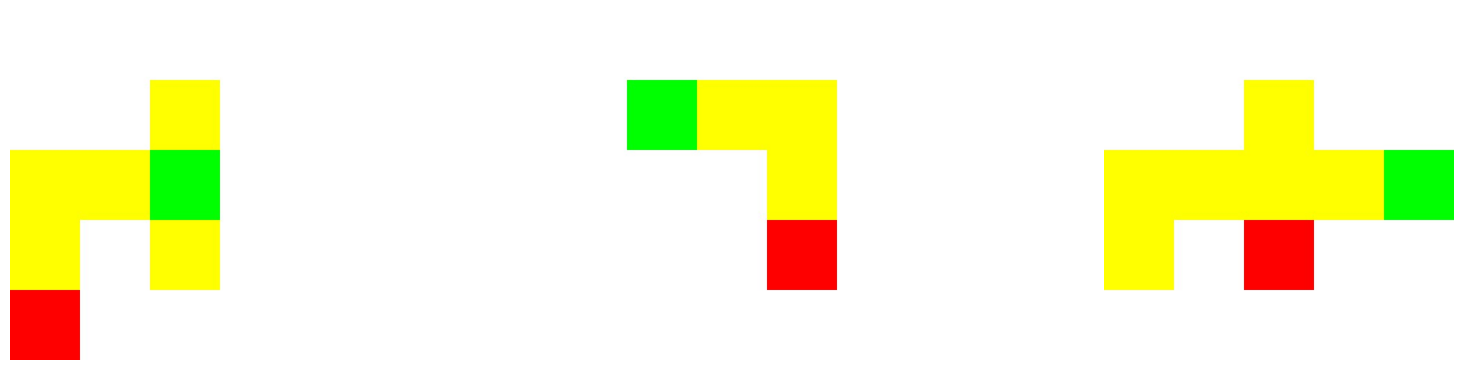
\includegraphics[width=0.75\textwidth]{images/genplanexperiment.png}
    \caption{Maze problems evaluated in the "Efficiency" experiment}
\end{figure}

\begin{figure}[h!]
    \centering
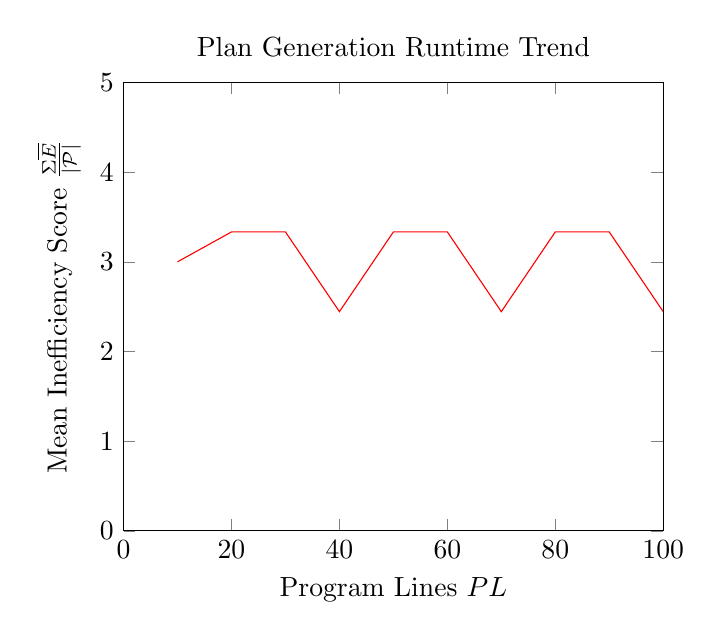
\begin{tikzpicture}
\begin{axis}[
    title={Plan Generation Runtime Trend},
    xlabel={Program Lines $PL$},
    ylabel={Mean Inefficiency Score $\frac{\Sigma\overline{E}}{|\mathcal{P}|}$},
    xmin=0, xmax=100,
    ymin=0, ymax=5,
]

\addplot[
    color=red,
    ]
    coordinates {(10, 3.0)(20, 3.3333333333333335)(30, 3.3333333333333335)(40, 2.4444444444444446)(50, 3.3333333333333335)(60, 3.3333333333333335)(70, 2.4444444444444446)(80, 3.3333333333333335)(90, 3.3333333333333335)(100, 2.4444444444444446)};
    
\end{axis}
\end{tikzpicture}
\caption{Plot of Mean Inefficiency Scores $T$}
\end{figure}

\subsection{Evaluation}
Overall, Figure 4.3 shows that there is \textit{not} a relationship between the program lines and plan efficiency, disproving the hypothesis. The optimal amount of plan lines for this problem is at 40, 70 or 100 where the mean inefficiency score is at its lowest. From this graph, at no point was a plan of any length classified as efficient enough. This could suggest that either the boundary for efficient generalised solutions is too high or that the planner cannot generate a plan efficient enough for this set of problems. This experiment can be carried out at a larger scale, taking into account the effect of a variety of problems, in future work. This evaluation was done due to the interest of understanding the consequence of modifying program lines in the synthesis of generalised plans.